\begin{problem}{범수크래프트}
	{standard input}{standard output}
	{3 seconds}{128 megabytes}{}
	
	지구이웨 마을에는 $n$개의 집이 $n-1$개의 도로로 연결되어있다. 모든 두 집에 대해서, 하나로 부터 다른 하나로 가는 경로가 유일하다. 집은 1번부터 $n$번까지의 번호가 붙어있다. 1번 집은 마을 이장 범수의 집이다. IoT(Internet of things)의 발달로 시골 마을에도 컴퓨터가 들어오게 되었고, $n$대의 컴퓨터가 범수의 집에 도착했다. 각 집에 하나씩 컴퓨터를 나눠주는게 범수의 일이다. 지구이웨 마을 사람들은 이미 게임 \textit{범수크래프트}를 하기로 약속한 상태이다.
	
	범수는 자신의 트럭에 모든 컴퓨터를 담고 나누어줄 준비를 했다. 범수는 정확히 각 도로를 왕복할 연료만 가지고 있다. 각 집에 가서 범수는 컴퓨터 하나를 내려 두고 바로 다음 집으로 간다. 각 집은 컴퓨터를 받으면 바로 컴퓨터를 켜서 범수크래프트를 설치한다. 범수크래프트를 설치하는 시간은 얼마나 기술에 익숙하냐에 따라 다르다. 범수는 모든 집에 컴퓨터를 배달하고 집에 와서 바로 범수크래프트를 설치할 것이다. 도로 하나를 다니는데 걸리는 시간은 정확히 1분이고, (범수크래프트를 하려는 의지 덕분에) 컴퓨터를 트럭에서 내리는 시간은 무시할 수 있다.
	
	범수를 도와서 범수를 포함한 모두가 최대한 빨리 범수크래프트를 같이 할 수 있게 도와주자. 즉, 모든 컴퓨터에 범수크래프트가 깔리는 데 필요한 최소 시간을 구하여라.
	
	\InputFile
	입력의 첫째 줄에는 지구이웨에 있는 집의 수 $n$이 주어진다. ($2 \le n \le 1,000,000$) 둘째 줄에는 $n$개의 정수 $c_1, c_2, \cdots, c_n$이 공백 하나로 구분되어 주어진다. ($1 \le c_i \le 10^9$) $d_i$는 $i$번째 집이 범수크래프트를 설치하는데 (분 단위로) 걸리는 시간이다.
	
	다음 $n-1$개의 줄에는 집을 잇는 도로를 설명한다. 각 줄은 두 정수 $a$, $b$가 공백 하나로 구분되어 주어진다. ($1 \le a < b \le n $) 이것은 $a$와 $b$를 직접 잇는 도로가 존재한다는 의미이다.
	
	
	\OutputFile
	
	프로그램은 하나의 수를 첫째 줄에 출력해야 한다. 이 수는 분 단위로 모두가 범수크래프트를 시작 할 수 있는 최소 시간이다.
	
	\SubtaskWithCost{1}{40}
	\begin{itemize}
		\item $n \le 7,000$
	\end{itemize}
	
	\SubtaskWithCost{2}{60}
	추가 제한 조건이 없다.
	
	
	
	\Examples
	
	\begin{example}
	\exmp{
	6
	1 8 9 6 3 2
	1 3
	2 3
	3 4
	4 5
	4 6
	}{%
	11
	}%
	\end{example}

\Notes

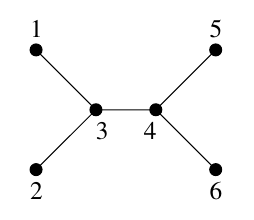
\includegraphics[]{far.png}

범수는 컴퓨터를 다음 순서로 배달해야 한다.: 3, 2, 4, 5, 6, 1. 게임은 각각 11, 10, 10, 10, 8, 9분 후에 깔릴 것이다. 그러므로 모두가 11분 후면 게임을 플레이 할 수 있다.

만약 범수가 3, 4, 5, 6, 2, 1 순서로 게임을 배달 했다면, 게임은 11, 16, 10, 8, 6 분 후에 깔릴 것이다. 그래서 모두가 16분 후에 게임을 플레이 해야 한다.

\end{problem}

